\documentclass[a4paper,twoside,master.tex]{subfiles}
\begin{document}
\lecture{31}{Friday, November 01, 2019}{Periodic Potentials}
Suppose $ V(x+a) = V(x) $. From a previous lecture, we introduced a translation operator $ (T_a V)(x) = V(x-a) = V(x)$ for periodic potentials, where $ T_a = e^{a\dv{x}} $.

We can see that the discrete translation over the period of the potential commutes with the Hamiltonian, $ \comm{T_a}{H} = 0 $. Recall that when we have an operator which commutes with the Hamiltonian, there exists a conserved charge. When we did this with infinitesimal translations, we found that the invariance leads to conservation of momentum. We can find the conserved charge here through Ehrenfest's theorem:
\begin{equation}
    \partial_t \expval{T_a} = \frac{1}{\imath \hbar} \expval{\comm{T_a}{H}} = 0
\end{equation}
Notice that our infinitesimal translation no longer commutes with the Hamiltonian, since $ (T_\epsilon V)(x) = V(x-\epsilon) \neq V(x) $. Momentum is no longer conserved in this case (not a free particle anymore). Something is still conserved here, but that thing is not momentum.

Let's see what happens when we have a plane wave in this periodic potential.
\begin{equation}
    \varphi(x, t=0) \equiv \varphi_0 = e^{\imath qx}
\end{equation}
If we translate the initial plane wave,
\begin{equation}
    (T_a \varphi_0)(x) = e^{- \imath q a} \varphi_0(x)
\end{equation}
we can look at the expectation value of the translation operator:
\begin{equation}
    \expval{T_a}{\varphi_0} = e^{-\imath qa}
\end{equation}
If we look at the wave function at time $ t $, we know that this matrix element is time-invariant from Ehrenfest's theorem, so
\begin{equation}
    \expval{T_a}{\varphi_t} = \expval{T_a}{\varphi_0}
\end{equation}
Therefore, $ e^{-\imath qa} $ is conserved! Note this doesn't imply that $ q $ is conserved. The exponential is invariant under $ q \to q + 2n \pi/a$. Any function that varies by $ e^{-\imath qa} $ under this translation must be periodic with a frequency of $ q + 2n\pi/a $. We claim this function has a Fourier series:
\begin{equation}
    \varphi(x,t) = \sum_{k} C_k(t) e^{\imath kx}
\end{equation}
where $ k = q + \frac{2 \pi}{a} n $. To clarify, an arbitrary wave function can be represented as a Fourier sum:
\begin{equation}
    \varphi(x,t) = \int \dd{k} C(k,t) e^{\imath kx}
\end{equation}
However, only discrete $ k $ values will be result in a wave function that transforms with this conserved charge.

What we discover then is that $ \hbar q $, the momentum, is not conserved, but the set $ \{q + \frac{2 \pi}{a} n\} $ is conserved. This is related to Bragg scattering. If an electron entered a crystal with momentum $ q $, it could exit with a momentum $ q + \frac{2 \pi}{a} n $, where $ a $ relates to the spacing of the crystal lattice. If we start with an initial plane wave, the thing that emerges after time evolution will be a function of the above form. There are non-vanishing Fourier modes for other values of $ k $, but they always belong to the conserved set. This is a weak conservation law, since a discrete periodic potential is actually a reduction of symmetry from a constant potential, which has a continuous symmetry. The higher symmetry of the constant potential conserves momentum absolutely while the discrete periodic potential allows for finite variations in the momentum. In terms of groups, we would say that the symmetry group for such a crystal is $ G = \{T_a^n, n \in \Z\} $. For the continuous symmetry group, we have $ \tilde{G} = \{T_a, a \in \R\} $.

This is a derivation of a more general statement called the Bloch Theorem:
\section{The Bloch Theorem}
\label{sec:the_bloch_theorem}
\begin{theorem}
    \begin{equation}
        \comm{T_a}{H} = 0 \implies \exists \text{ simultaneous eigenfunctions}
    \end{equation}
\end{theorem}

Let's look at the translation of a more general function:
\begin{align}
    T_a \left[ e^{\imath q x} U(x) \right] &=  e^{-\imath q a} \left[ e^{\imath qx} U(x-a) \right]\\
    &= e^{-\imath qa} \left[ e^{\imath q x} U(x) \right]
\end{align}
if $ U(x-a) = U(x) $ is periodic. Therefore, the eigenstates of the Hamiltonian are of the form $ e^{\imath qx} U(x) $.

For our previous example, we had
\begin{equation}
    \varphi(x, t) = e^{\imath q x} \underbrace{\sum_j C_j(t) e^{\frac{2 \pi \imath jx}{a}}}_{U(x)}
\end{equation}
Typically there is dependence of $ U(x) $ on $ q $, so $ U(x) = U(x,q) = U_q(x) $. Because they are eigenstates,
\begin{equation}
    H \varphi_q = E(q) \varphi_q
\end{equation}
and for a given $ q $ there could be more than one such function that gives an eigenstate of the Hamiltonian. We will add another index $ s $ which we will call the ``band'' index in addition to $ q $ which we call the ``Bloch'' index:
\begin{equation}
    H \psi_{q,s} = E_s(q) \psi_{q,s}
\end{equation}
Below is a plot of the energy eigenstates as functions of $ q $. This is called the band structure of the eigenstate:
\begin{figure}[h]
    \centering
    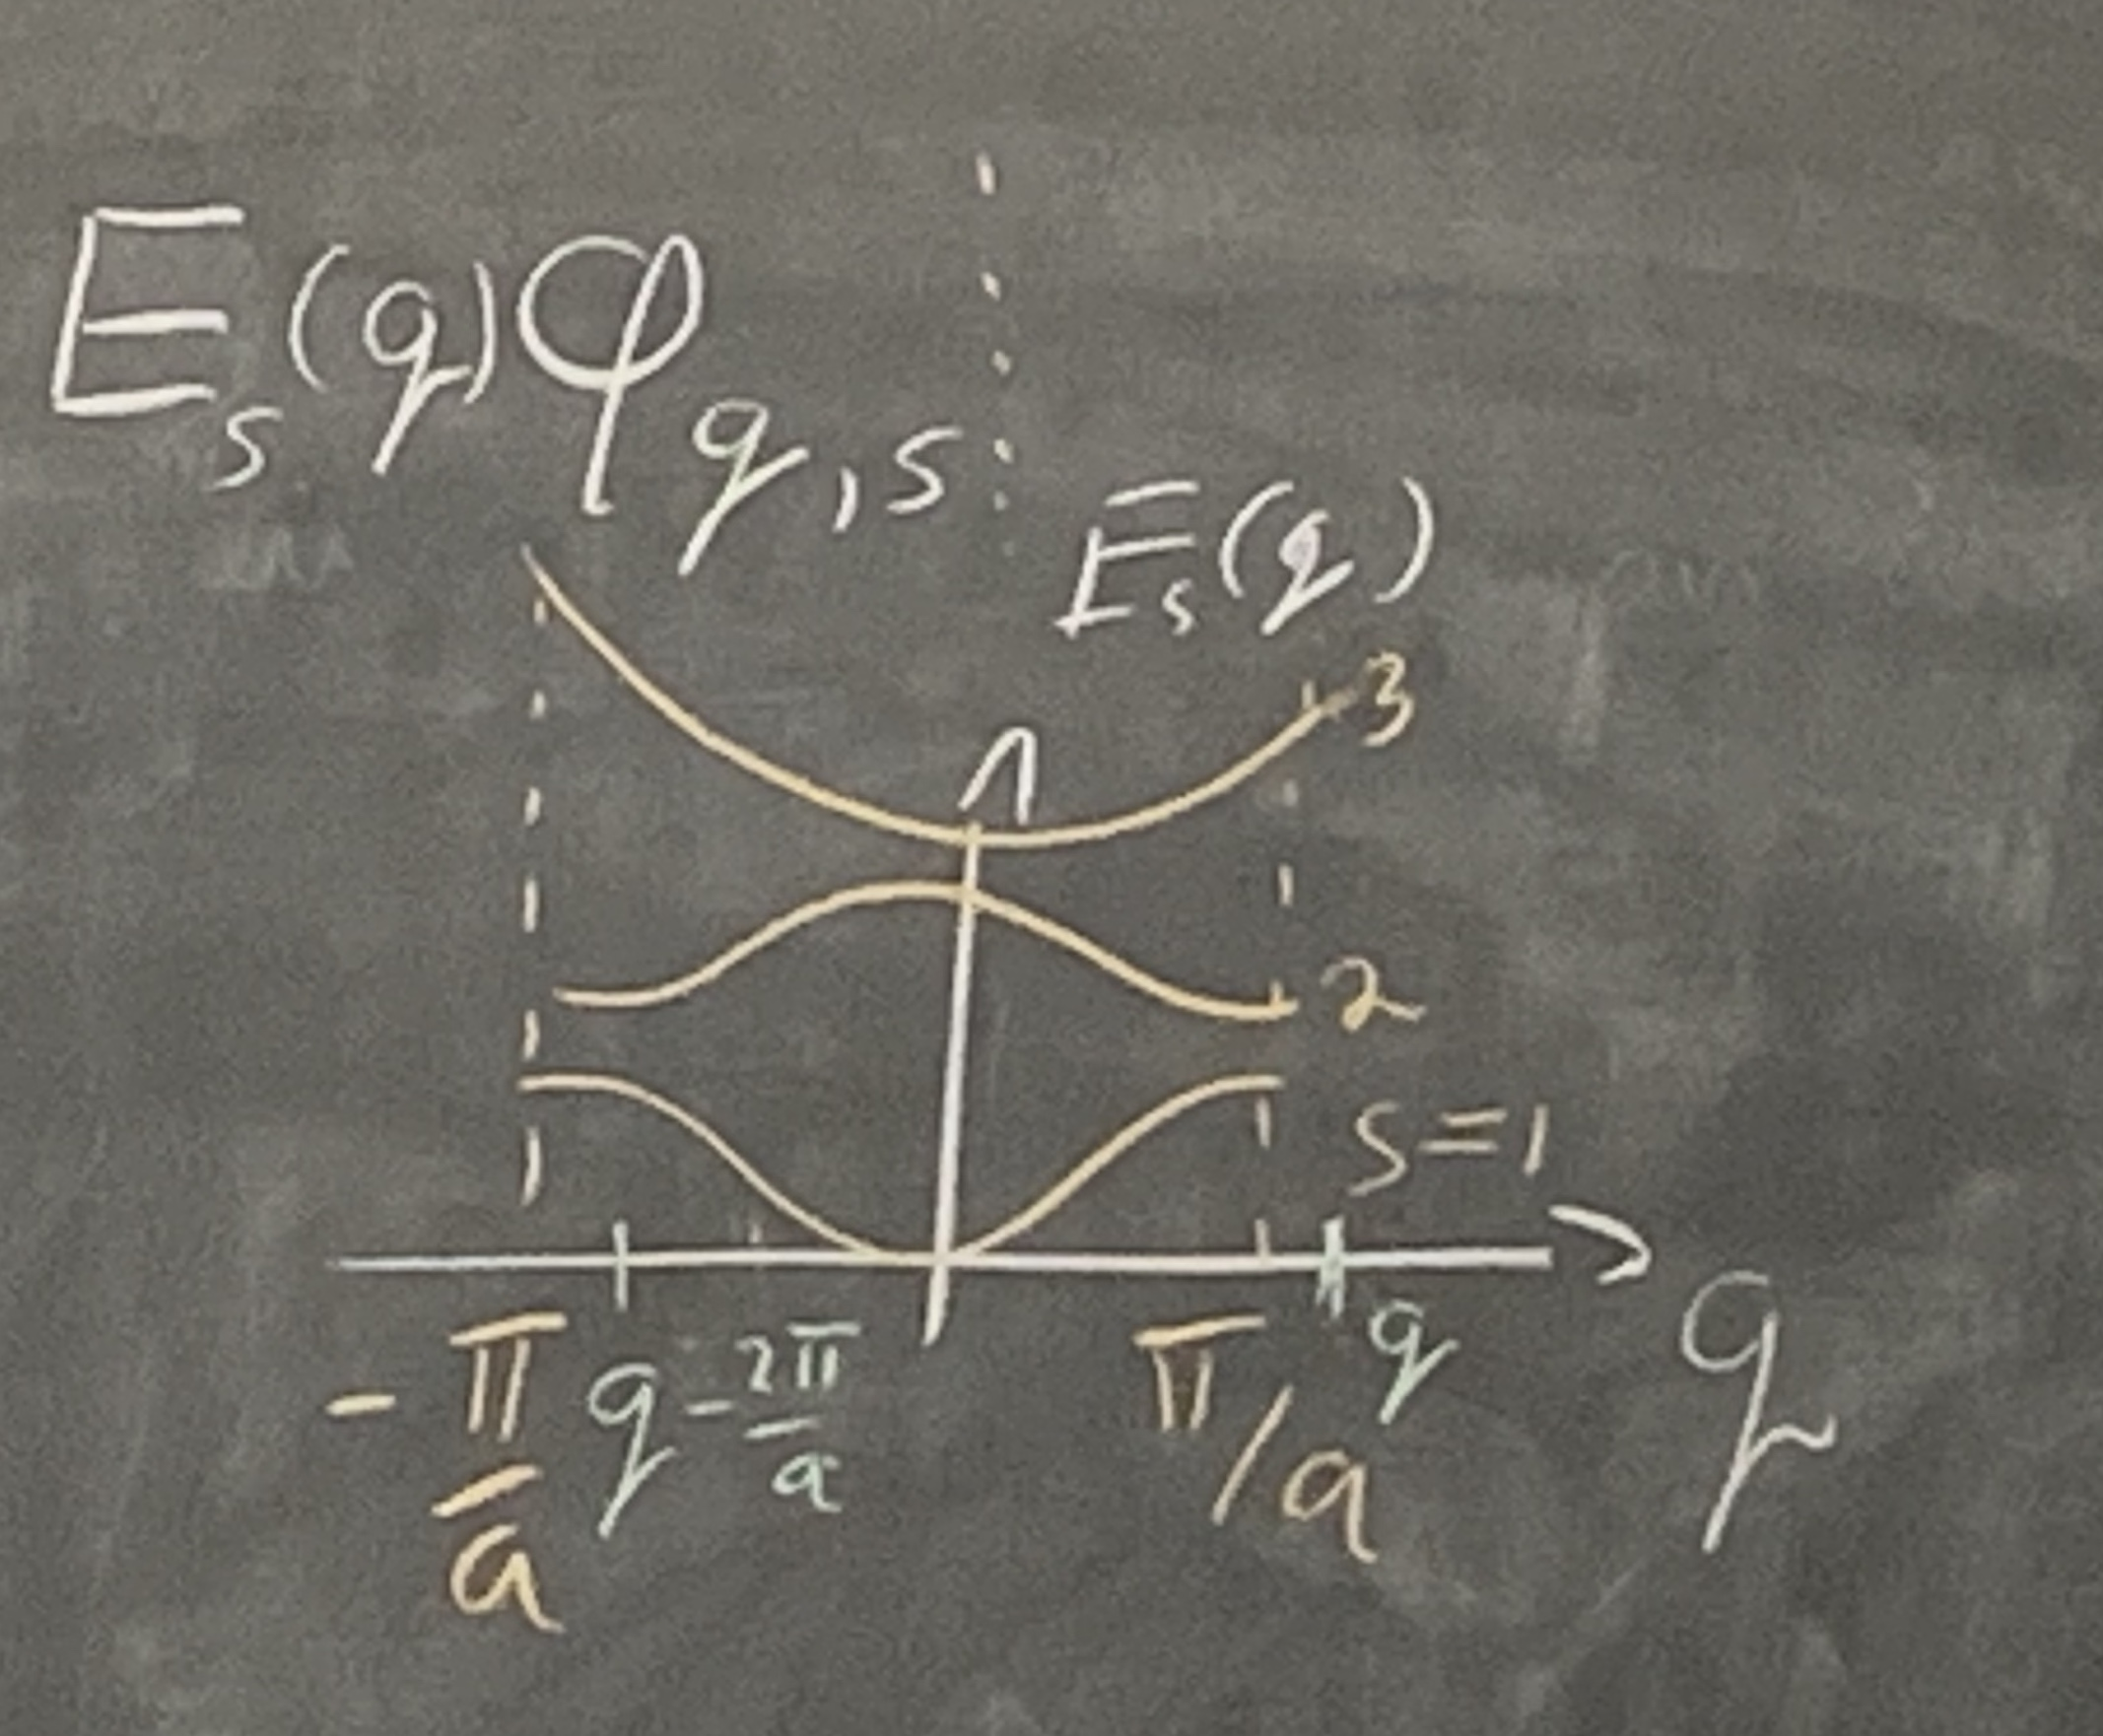
\includegraphics[width=\textwidth/2]{figures/lec_31_band.jpg}
    \caption{Example Band Structure}
    \label{fig:example_band_structure}
\end{figure}




\end{document}
